%\documentclass[a4paper]{article}
%\usepackage{beamerarticle}

\documentclass[ignorenonframetext]{beamer}
\usepackage{beamerthemesplit}
\usepackage{amssymb}

\usepackage{../fhnw-beamer}

%\mode<article>{\usepackage{fullpage}}
%\mode<presentation>{\usetheme{Berlin}}

\date{\today}
\author{rolf.schmutz@fhnw.ch}
\institute{FHNW}
\title {Netzwerke und Datenkommunikation\\NDK 02-050\\Layer-4 UDP \& TCP}


\begin{document} % ===============================================================

\section{NDK 02-050: 7}



\begin{frame}
\titlepage
\end{frame}




\begin{frame}
\frametitle{Ziele}
\begin{itemize}
	\item{Sie kennen die Transportschichtprotokolle UDP und TCP und geeignete Anwendungen}
	\item{Sie kennen die Software-Abstraktion ``Socket'' und das dazugeh\"orige demultiplexing auf dem System}
	\item{Sie k\"onnen Verbindungen auf dem System identifizieren}
\end{itemize}
\end{frame}



\begin{frame}
\frametitle{Layer-4: Transportschicht 1/2}
\begin{itemize}
	\item{Die Schicht 4 f\"uhrt eine Abstraktion f\"ur Kommunikationskan\"ale ein, die die unterliegende Paketschicht verbirgt}
	\item[1]{Es gibt einen verbindungslosen ``Telegrammdienst'' (UDP) f\"ur kurze und/oder ``einweg'' Meldungen\footnote{$\ldots$ziemlich genaue Analogie}}
	\item[2]{$\ldots$ und einen verbindungsorientierten, bidirektionalen Dienst mit garantierter Sequenz\footnote{analog z.B. einer Telefonverbindung}}
\end{itemize}
	\begin{block}{Abstraktion}
\textbf{beides sind ``Illusionen'', die die paketorientierte Arbeitsweise von IP verbergen}\\
auf beiden Endger\"aten muss ein Verbindungsstatus gepflegt werden
\end{block}
\end{frame}


\begin{frame}
\frametitle{Layer-4: Transportschicht 2/2}
\begin{itemize}
  \item{Server: SAPI \emph{passive-open} \texttt{accept} (warte auf Anfragen)}
  \item{Client: SAPI \emph{active-open} \texttt{connect} (startet eine Anfrage)}
  \item{Beide: SAPIs \emph{send, receive, close} (Datenkommunikation)}
\end{itemize}
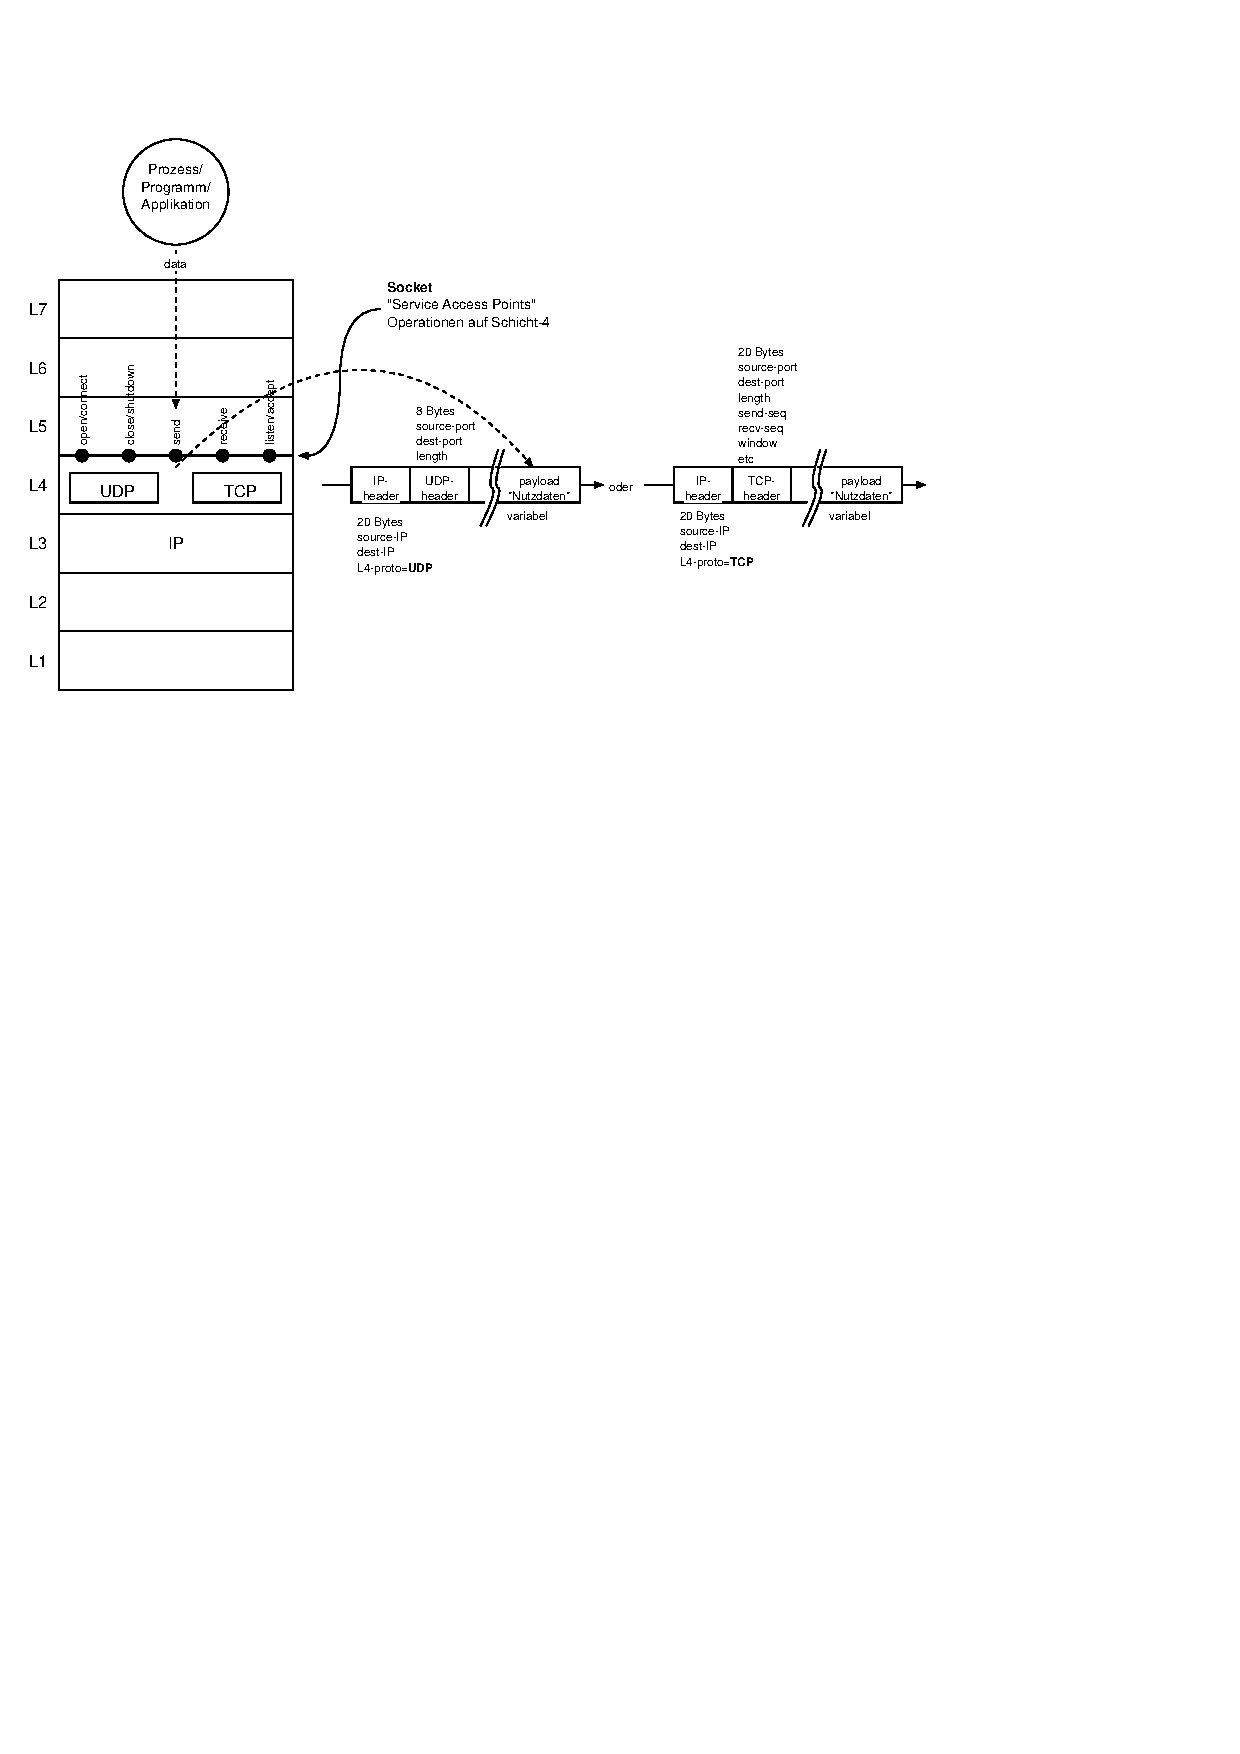
\includegraphics[height=17cm]{stack}
\end{frame}


\begin{frame}
\frametitle{UDP: User Datagram Protocol}
\begin{itemize}
	\item{kann f\"ur kurze Einwegmeldungen\footnote{d.h. ohne Best\"atigungsmeldung, best-effort} wie z.B. Systemlog\footnote{Windows: {\em Eventlog}, Transkript}}
	\item{oder auch f\"ur bidirektionale Konversation\footnote{{\em request} und {\em reply}} wie z.B. DNS/Verzeichnisdienst\footnote{$\ldots$damit Sie \texttt{www.eff.org} eingeben k\"onnen und DNS findet dann die IP-Adresse \texttt{64.147.188.3} dazu}}
	 verwendet werden
	 \item{es ist Aufgabe der Applikation\footnote{Prozess/``Programm'', auf Server- und Client-Seite} Antwort-Datagramme zu senden -- UDP selbst ``kennt'' das jeweilige Schicht-7 Protokoll nicht}
	 \item{unterst\"utz {\em Multicasting} -- senden von Daten an viele Hosts gleichzeitig}
	 \item{die Bezeichnung f\"ur eine Dateneinheit (Telegramm) ist {\em datagram}}
\end{itemize}
\begin{block}{Telegrammdienst}
\textbf{Die jeweiligen Applikationen/Programme\footnote{{\em client} und {\em server}} m\"ussen die eventuelle Quittierung oder Wiederholung von Meldungen selber sicherstellen}
\end{block}
\end{frame}

\begin{frame}
\frametitle{UDP Communication}
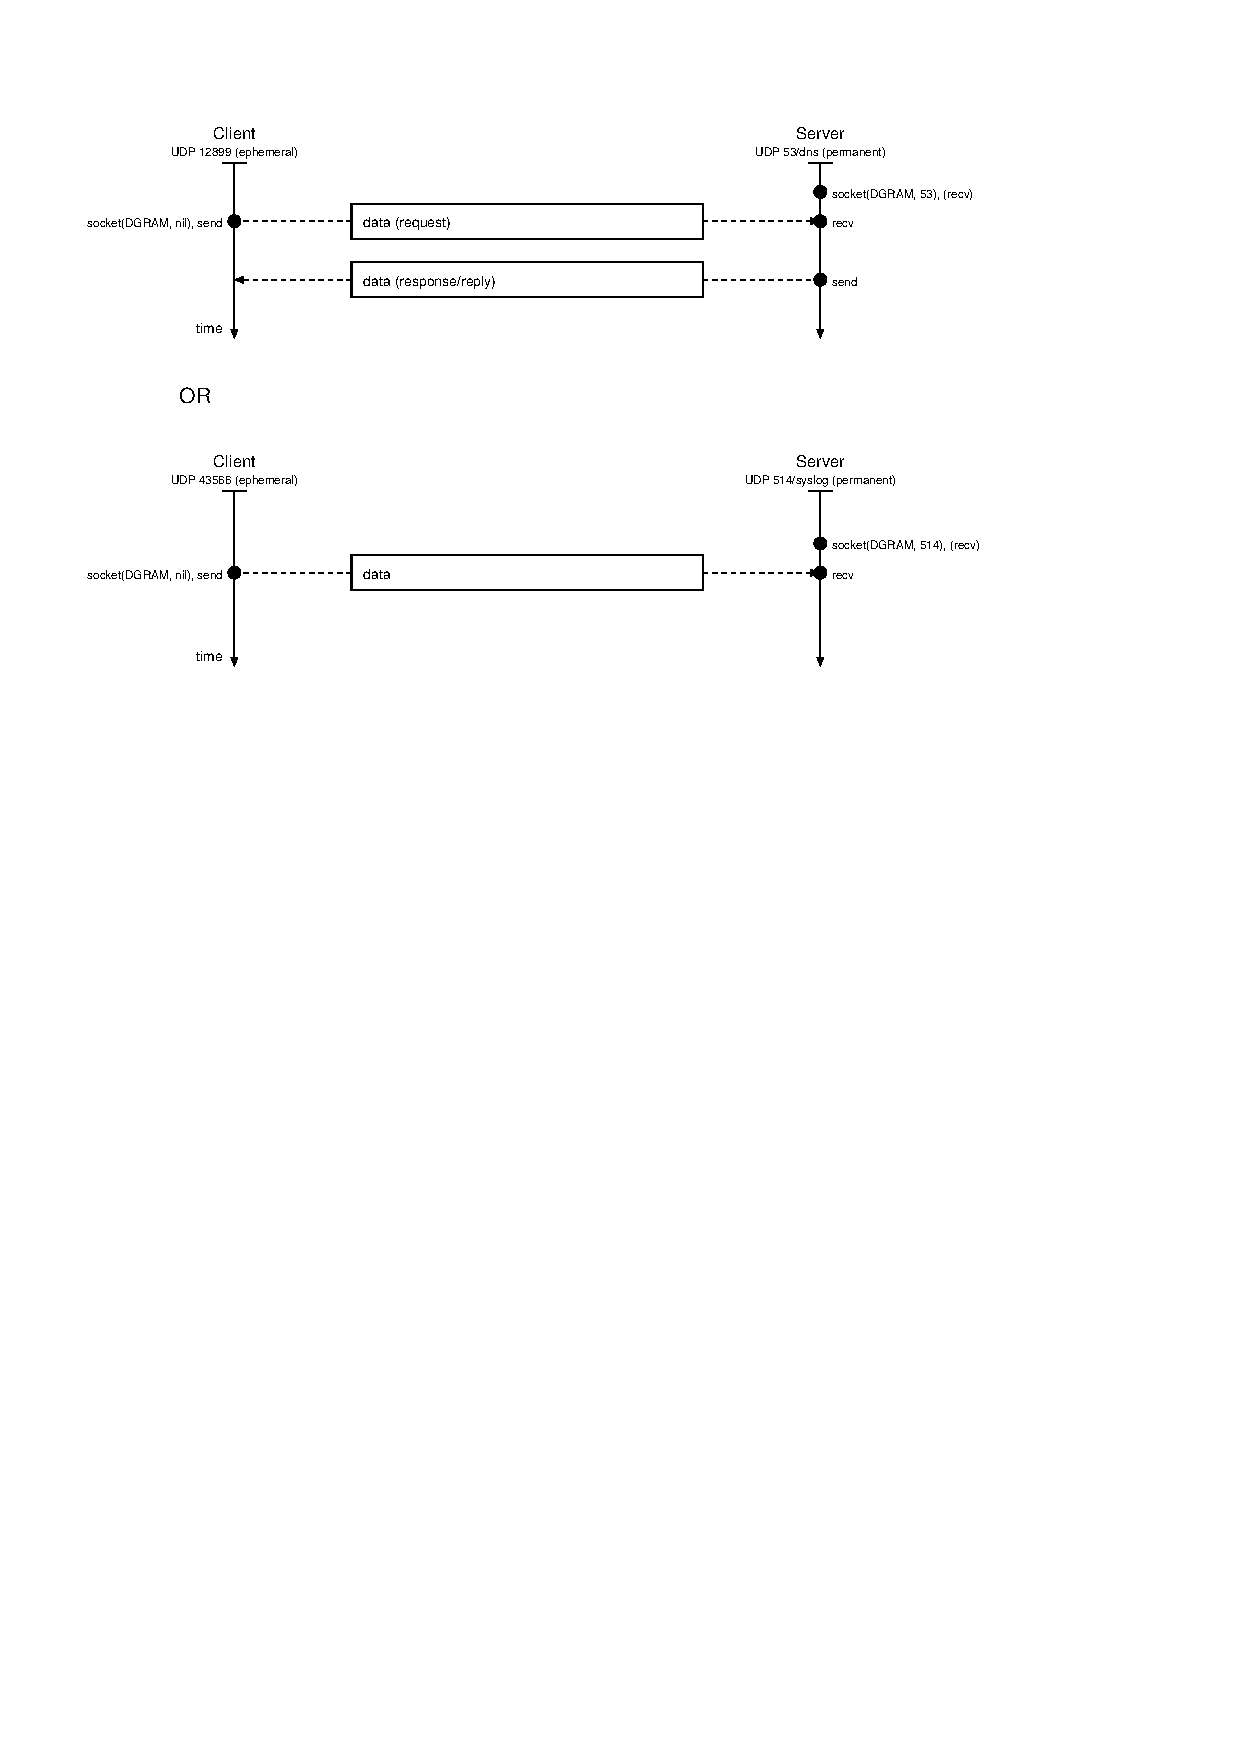
\includegraphics[width=15cm]{udp-communication}
\end{frame}




\begin{frame}
\frametitle{TCP: Transmission Control Protocol 1/5}
\begin{itemize}
	\item{Zweiweg\footnote{bidirektional} verbindungsorientierte Kommunikation}
	\item{garantierte Sequenz der Daten\footnote{auch wenn sich Pakete im Internet ``\"uberholen''}}
	\item{verlorene Pakete werden neu gesendet}
	\item{{\em Flusskontrolle} -- Empf\"anger kann ``stop'' oder ``langsamer senden'' verlangen}
	\item{die Bezeichnung f\"ur eine Dateneinheit ist {\em segment} -- allerdings ist die Abstraktion f\"ur die Software ein {\em stream} (Datenstrom)}
\end{itemize}
\begin{block}{Verbindungsorientierter Dienst}
\textbf{Transparente\footnote{d.h. die Client- und Server-Applikationen k\"ummern sich nicht um Paketwiederholungen, Sequenz, etc} bidirektionale (Richtungsgetrennt) Verbindung\footnote{\textbf{das ist eine nur eine ``Illusion'' -- die darunterliegende Schicht IP ist {\em nicht} Verbindungsorientiert}}}
\end{block}
\end{frame}


\begin{frame}
\frametitle{TCP Handshake, Session 2/5}
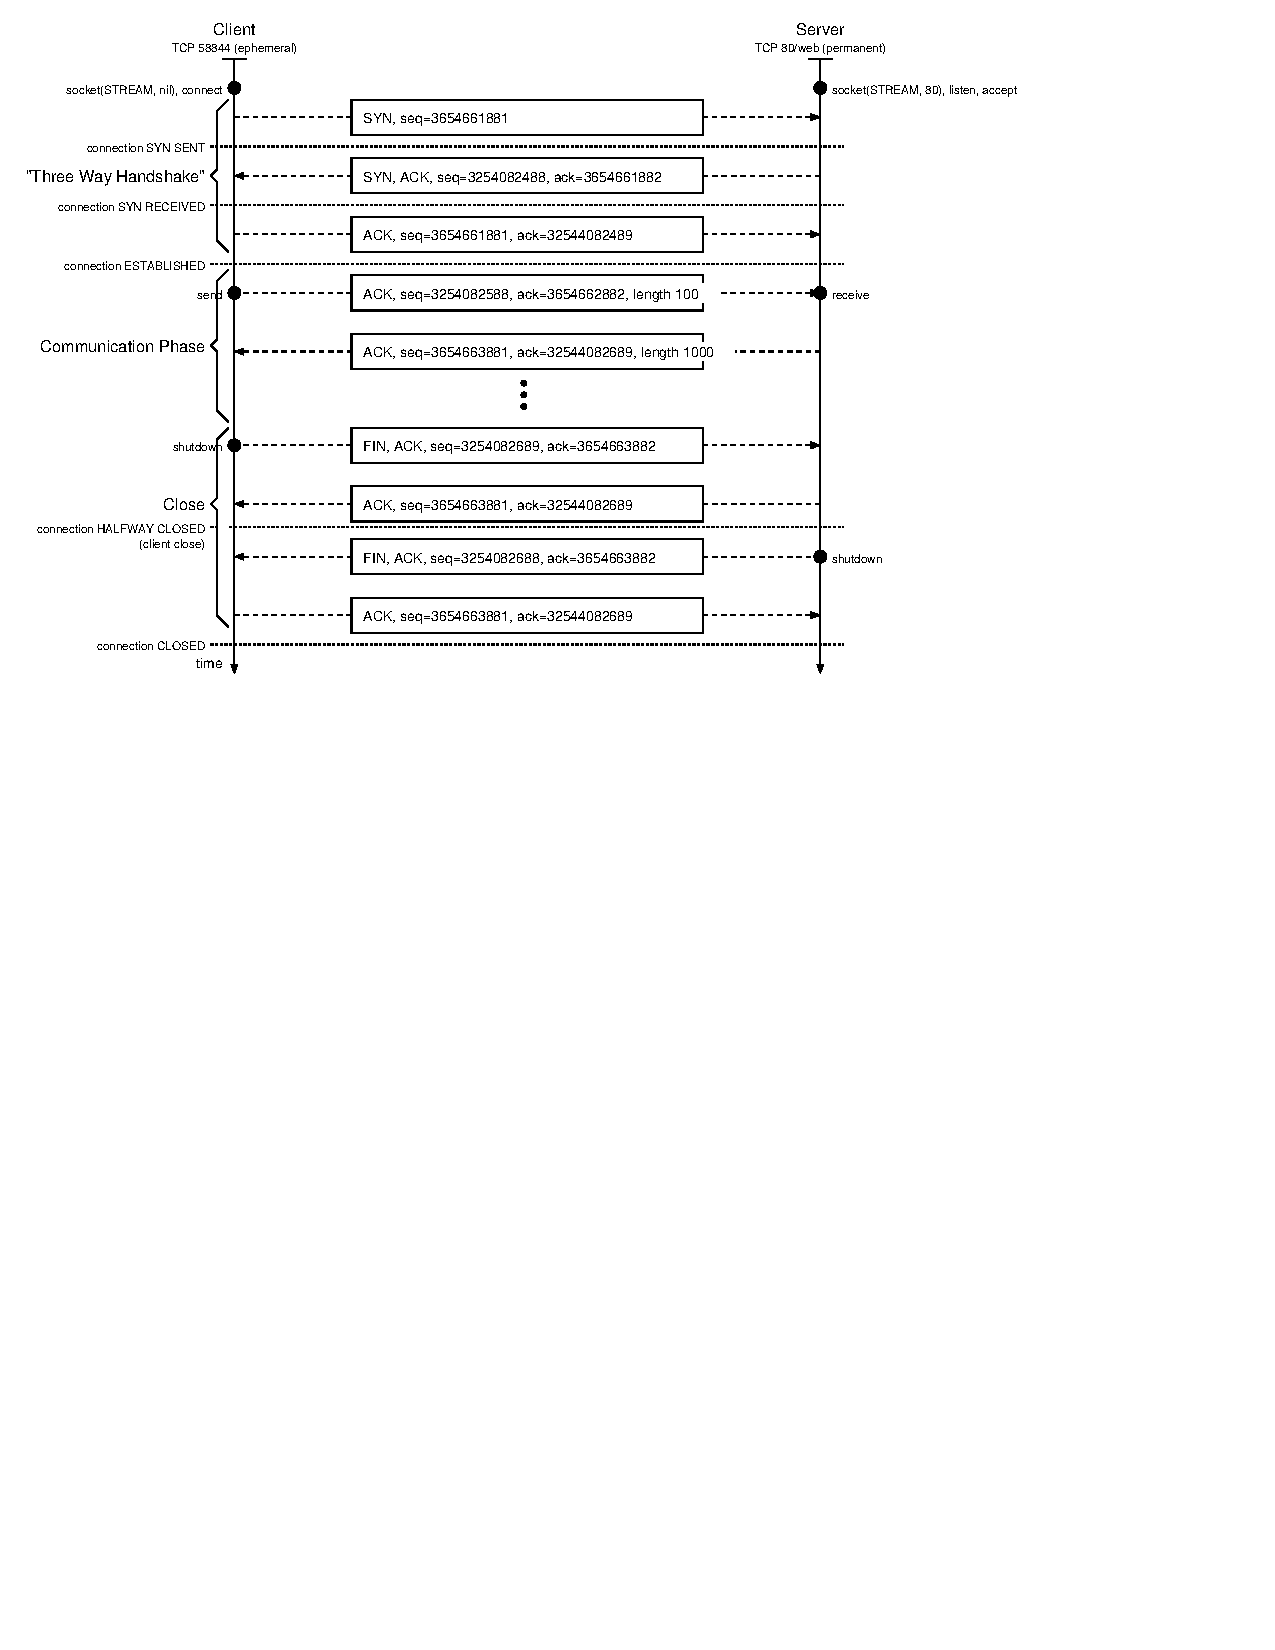
\includegraphics[width=15cm]{tcp-handshake}
\end{frame}


\begin{frame}
\frametitle{TCP Sequence, Window\footnote{\myurl{http://upload.wikimedia.org/wikipedia/commons/thumb/d/db/Tcp.svg/600px-Tcp.svg.png}} 3/5}
\begin{center}
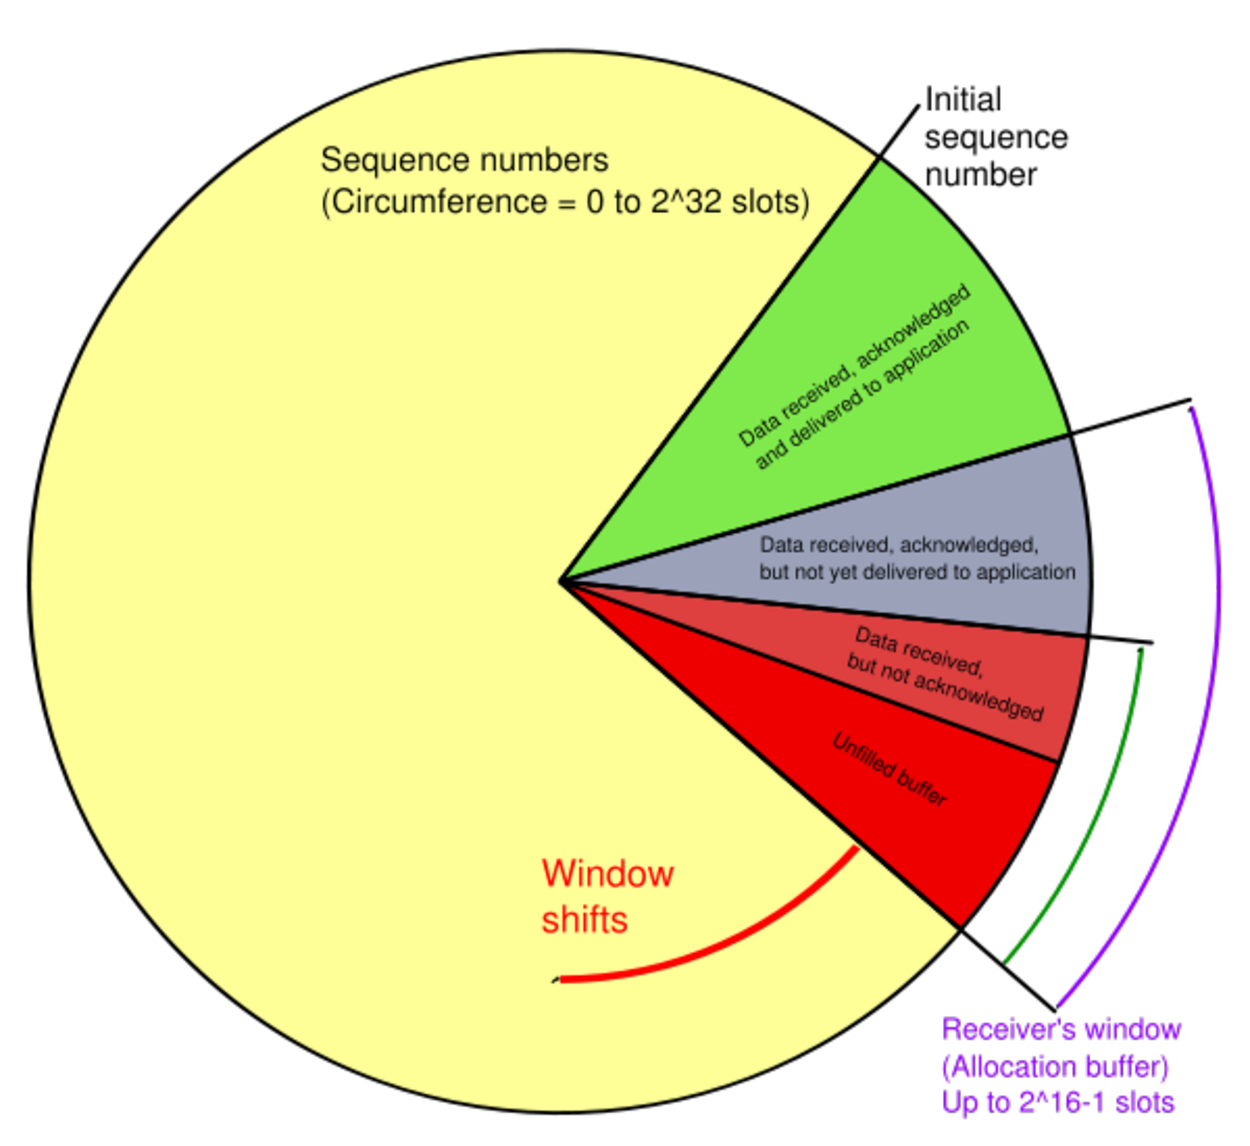
\includegraphics[width=8cm]{tcp-window}
\end{center}
\end{frame}

\begin{frame}
\frametitle{TCP Stati\footnote{\myurl{http://upload.wikimedia.org/wikipedia/commons/thumb/a/a2/Tcp_state_diagram_fixed.svg/796px-Tcp_state_diagram_fixed.svg.png}} 4/5}
\begin{center}
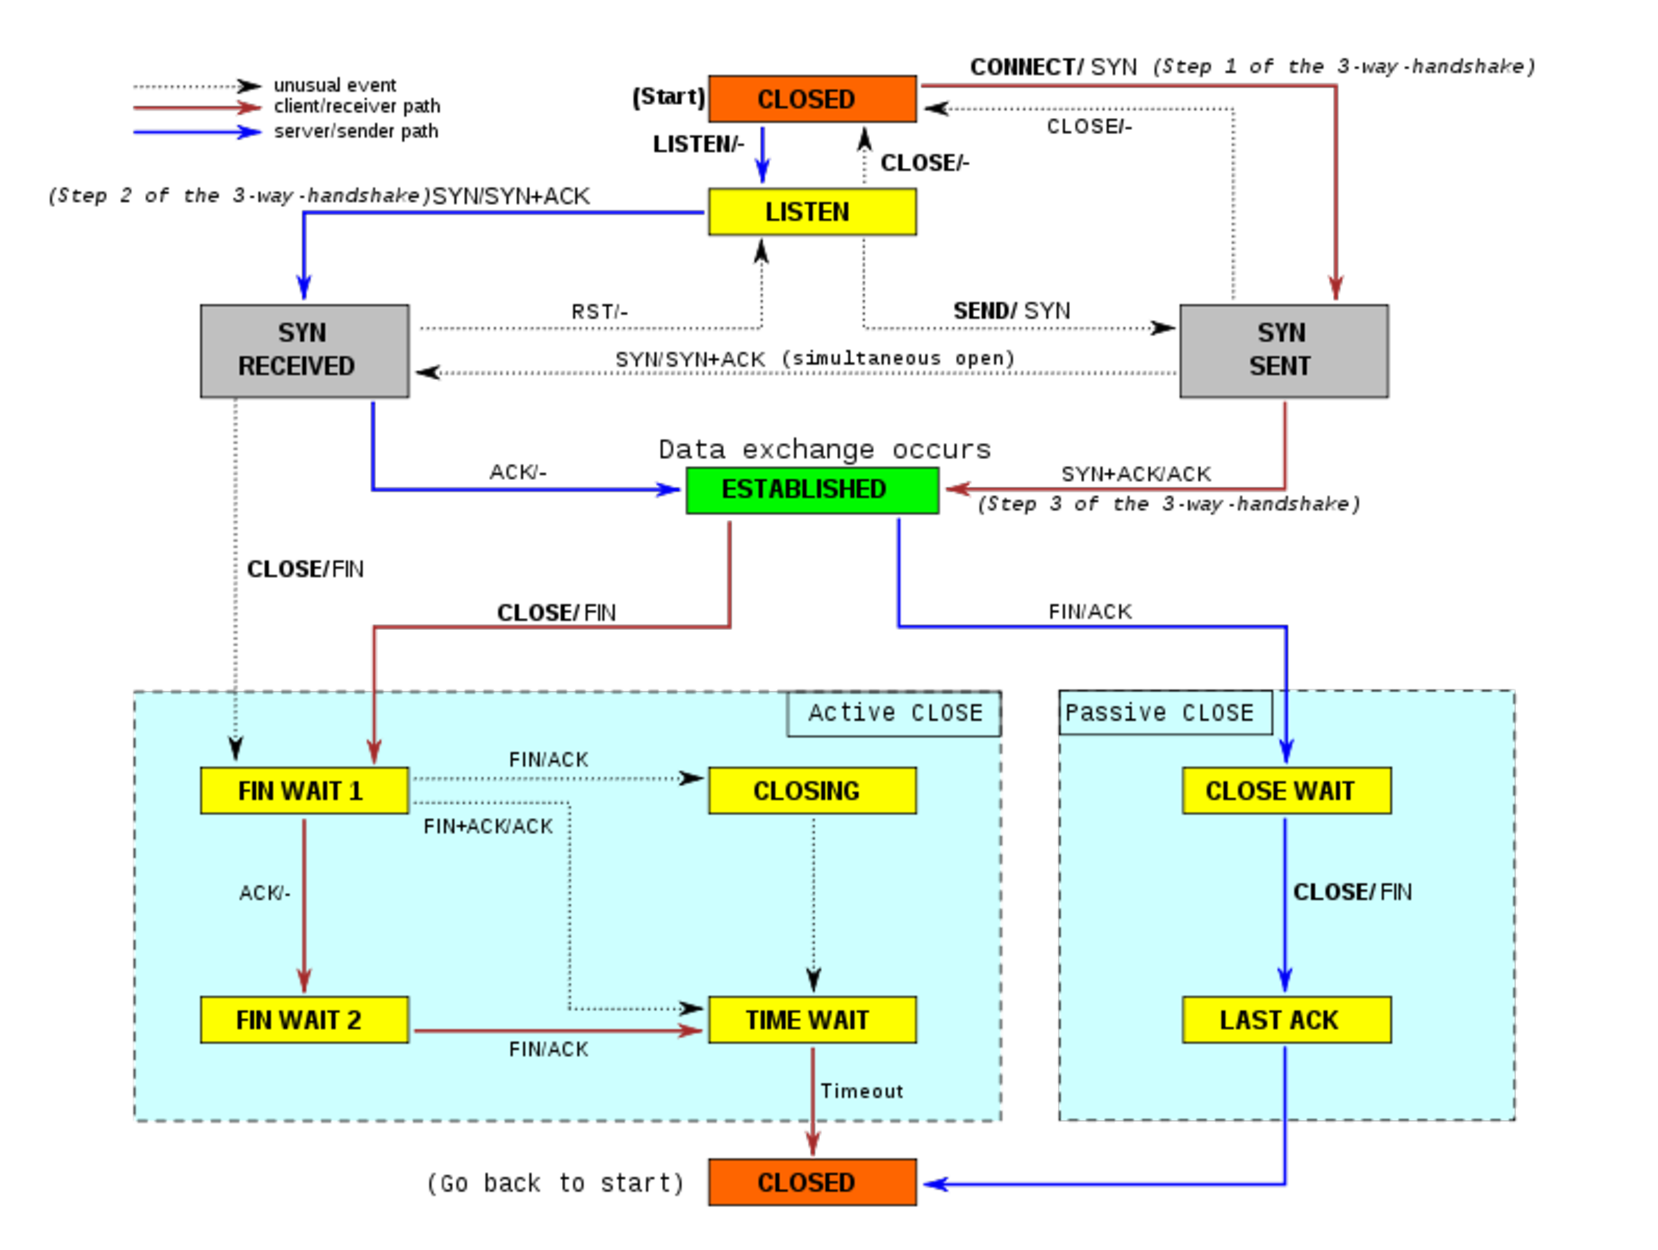
\includegraphics[width=9cm]{tcp-state-diagram}
\end{center}
\end{frame}


\begin{frame}[fragile]
\frametitle{TCP \texttt{tcpdump}{}\footnote{\texttt{sudo tcpdump -v -nnn -S -i en1 tcp port 80 and ip host zaphod} und dann \texttt{telnet zaphod 80}} (edited) 5/5}
\begin{tiny}
\begin{verbatim}
--- three-way handshake ---
19:09:56.361262 IP 10.202.5.121.63505 > 188.40.65.199.80: Flags [S], seq 1704735491, win 65535, length 0
19:09:56.384815 IP 188.40.65.199.80 > 10.202.5.121.63505: Flags [S.], seq 4146040110, ack 1704735492,
                win 5792, length 0
19:09:56.384871 IP 10.202.5.121.63505 > 188.40.65.199.80: Flags [.], ack 4146040111, win 33304, length 0

--- communication phase ---
19:10:00.891376 IP 10.202.5.121.63505 > 188.40.65.199.80: Flags [P.], seq 1704735492:1704735509,
                ack 4146040111, win 33304, length 17
19:10:00.915173 IP 188.40.65.199.80 > 10.202.5.121.63505: Flags [.], ack 1704735509, win 46, length 0
19:10:06.987161 IP 10.202.5.121.63505 > 188.40.65.199.80: Flags [P.], seq 1704735509:1704735533,
                ack 4146040111, win 33304, length 24
19:10:07.010497 IP 188.40.65.199.80 > 10.202.5.121.63505: Flags [.], ack 1704735533, win 46, length 0
19:10:07.531102 IP 10.202.5.121.63505 > 188.40.65.199.80: Flags [P.], seq 1704735533:1704735535,
                ack 4146040111, win 33304, length 2
19:10:07.555122 IP 188.40.65.199.80 > 10.202.5.121.63505: Flags [.], ack 1704735535, win 46, length 0
19:10:07.555127 IP 188.40.65.199.80 > 10.202.5.121.63505: Flags [P.], seq 4146040111:4146040348,
                ack 1704735535, win 46, length 237
19:10:07.555182 IP 10.202.5.121.63505 > 188.40.65.199.80: Flags [.], ack 4146040348, win 33185, length 0

--- shutdown ---
19:10:12.792188 IP 188.40.65.199.80 > 10.202.5.121.63505: Flags [F.], seq 4146040348,
                ack 1704735535, win 46, length 0
19:10:12.792244 IP 10.202.5.121.63505 > 188.40.65.199.80: Flags [.], ack 4146040349, win 33304, length 0
19:10:12.792341 IP 10.202.5.121.63505 > 188.40.65.199.80: Flags [F.], seq 1704735535,
                ack 4146040349, win 33304, length 0
19:10:12.815841 IP 188.40.65.199.80 > 10.202.5.121.63505: Flags [.], ack 1704735536, win 46, length 0
\end{verbatim}
\end{tiny}
\end{frame}



\begin{frame}[fragile]
\frametitle{Kommunikationsendpunkt ``Socket''}
\begin{itemize}
	\item{am weitesten verbreitete Software-Abstraktion eines Kommunikationsenpunkts ``Berkeley Socket''{}\footnote{von UC Berkley, BSD ``Berkeley Software Distribution''
	UNIX}}
	\item{ein Verbindungsversuch auf {\em closed ports}{}\footnote{kein Serverprozess} wird bei TCP mit einem RESET bei UDP mit einem ICMP-Port-Unreachable beantwortet}
	\item{der Kommunikationskanal wird von der Software wie eine Datei angesprochen\footnote{{\em read} und {\em write}. Bei TCP zus\"atzlich {\em open} und {\em close}}}\\
	\begin{tiny}
	\begin{verbatim}
root@zaphod:~# netstat -tunap4
Active Internet connections (servers and established)
Proto Recv-Q Send-Q Local Address           Foreign Address         State       PID/Program name
tcp        0      0 0.0.0.0:993             0.0.0.0:*               LISTEN      7720/imap-login 
tcp        0      0 0.0.0.0:80              0.0.0.0:*               LISTEN      19994/lighttpd  
tcp        0      0 127.0.0.1:53            0.0.0.0:*               LISTEN      32004/named     
tcp        0      0 0.0.0.0:22              0.0.0.0:*               LISTEN      3097/sshd       
tcp        0      0 0.0.0.0:25              0.0.0.0:*               LISTEN      1602/master     
tcp        0      0 0.0.0.0:443             0.0.0.0:*               LISTEN      19994/lighttpd  
tcp        0      0 188.40.65.199:22        77.56.89.75:45753       ESTABLISHED 18655/sshd: tunnel 
tcp        0      0 188.40.65.199:22        212.60.51.243:40469     ESTABLISHED 5604/sshd: tunnel
tcp        0      0 188.40.65.199:22        212.60.51.243:46973     ESTABLISHED 24007/sshd: tunnel 
tcp        0   3248 188.40.65.199:22        77.56.89.75:52550       ESTABLISHED 24992/sshd: rschmutz
tcp        1      0 188.40.65.199:80        77.56.89.75:51856       CLOSE_WAIT  19994/lighttpd  
udp        0      0 188.40.65.199:53        0.0.0.0:*                           32004/named     
udp        0      0 188.40.65.199:123       0.0.0.0:*                           3057/ntpd       
	\end{verbatim}
	\end{tiny}
\end{itemize}
\end{frame}


\begin{frame}
\frametitle{Layer-4: {\em Demultiplexing}}
\begin{tiny}
f\"ur das Demultiplexing wird
das 5-Tuple
\texttt{\{ protocol, local-ip, local-port, remote-ip, remote-port \}}
verwendet
\end{tiny}
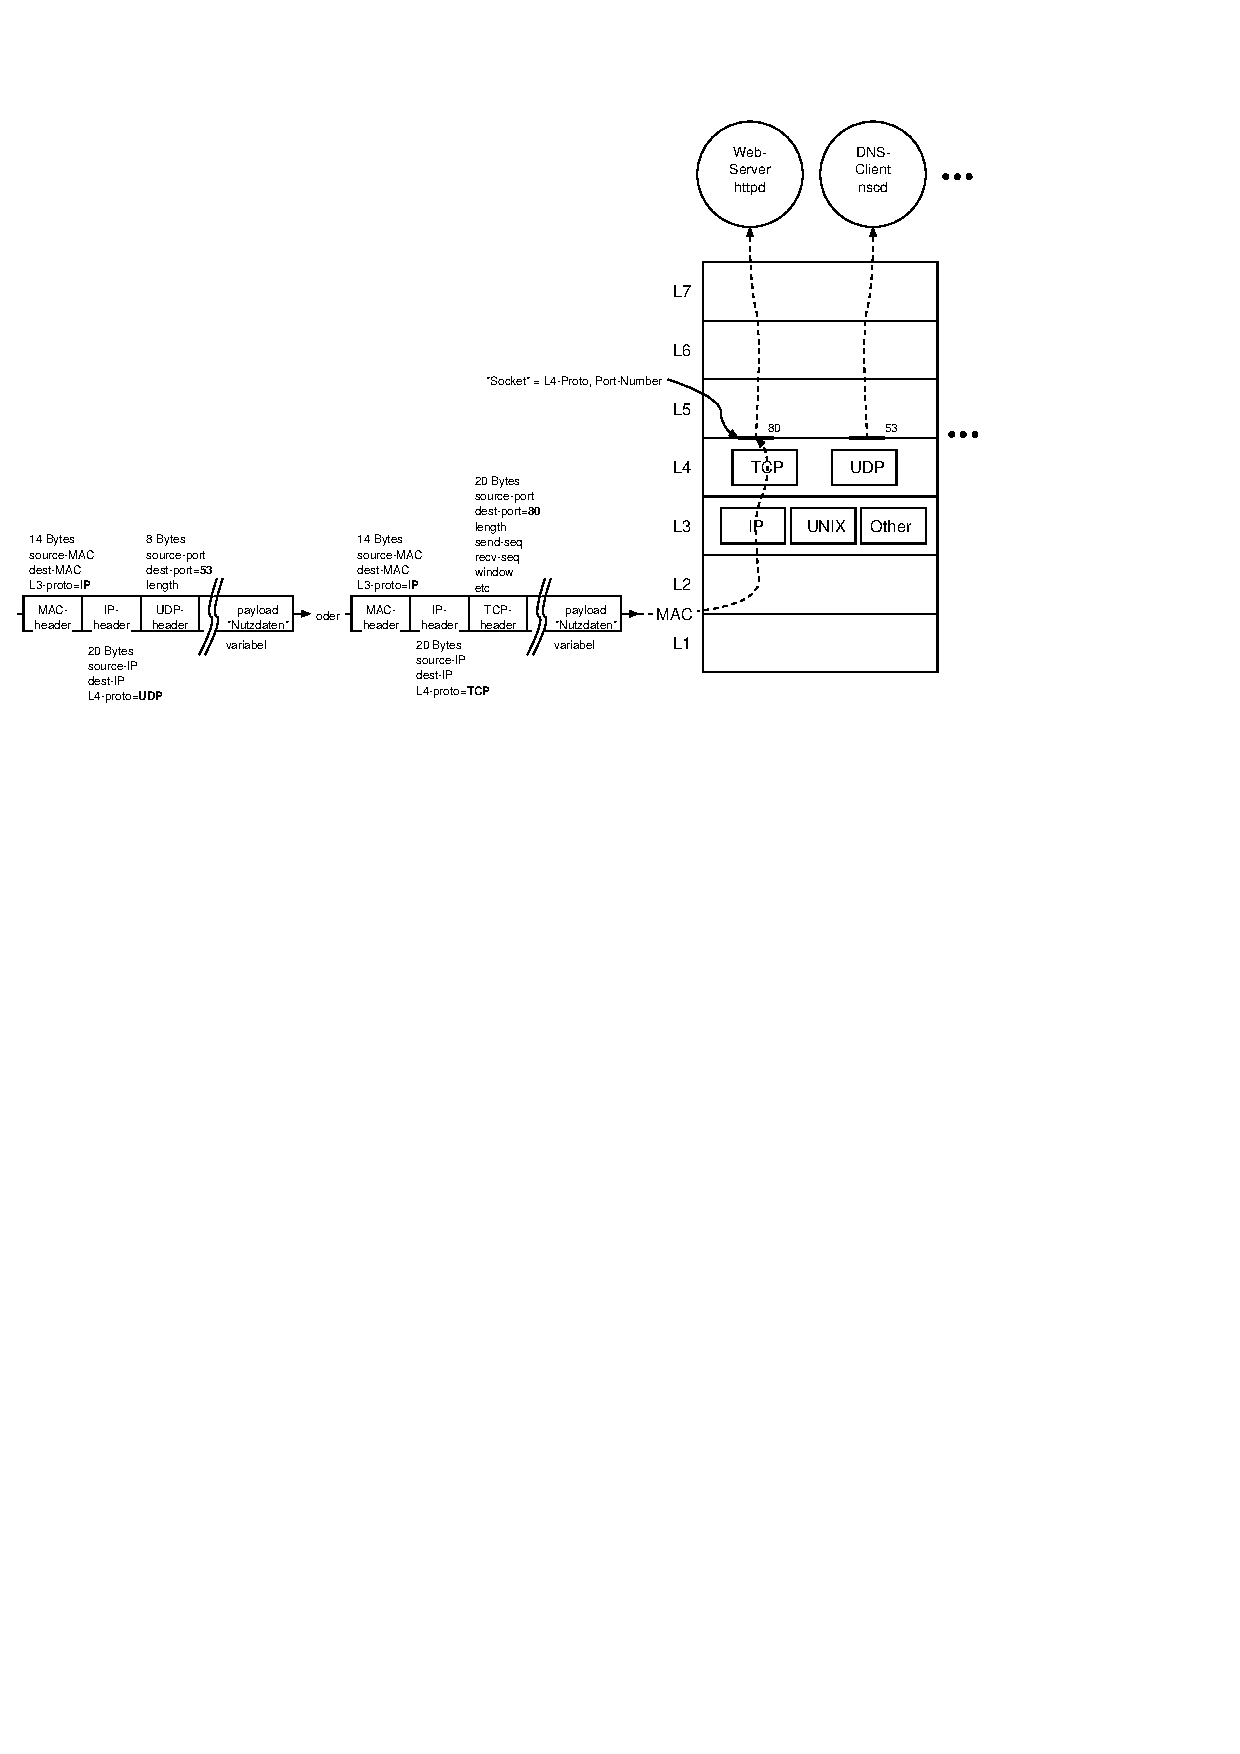
\includegraphics[height=6.5cm]{demultiplexing}
\end{frame}


\begin{frame}
\myurl{http://www-01.ibm.com/support/docview.wss?uid=isg1II12449}
\frametitle{Socket Stati\footnote{``Stat\"usser''}}
\end{frame}



\begin{frame}
\frametitle{Port Nummern\footnote{\myurl{http://en.wikipedia.org/wiki/TCP_and_UDP_port_numbers}} $\approx$ Dienst}
\begin{itemize}
	\item{um einen bestimmten Dienst\footnote{z.B. Web oder Mail} anzusprechen m\"ussen die die entsprechenden Portnummern bekannt sein}
	\item{Systemseitig werden anstatt Portnummern oft symbolische Namen benutzt\footnote{UNIX: \texttt{/etc/services} und \texttt{getent services {\em mail}} oder \texttt{getent services 25}}, Windows: \texttt{C:\\}}
	\item{Portnummern werden von IANA\footnote{Internet Assigned Numbers Authorithy,  \myurl{http://www.iana.org/assignments/port-numbers}} verwaltet}\\es gibt die
	\item[1]{{\em well-known-services}{}\footnote{``WKS'' auch bekannt als ``low-ports''} 0 bis 1023}
	\item[2]{{\em registered ports} 1024 bis 49151: darin finden sich bekannte Dienste (``Server-side'', {\em permanent}) aber auch ``Client-side'' ({\em ephemeral} Ports}
\end{itemize}
\end{frame}

\begin{frame}
\frametitle{Command Line Tools}
\begin{itemize}
	\item{Socket Status, ``offene Ports'': \texttt{netstat -an} (alle sockets)}
	\item{TCP Verbindungstest: \texttt{telnet {\em host} {\em port}}}
\end{itemize}
\end{frame}


\begin{frame}
\frametitle{References}
\begin{itemize}
	\item{Internet Standards: \myurl{http://tools.ietf.org/html/rfc1280}}
	\item{UDP:\\RFC \myurl{http://tools.ietf.org/html/rfc768} und\\Standard \myurl{http://tools.ietf.org/html/std6}}
	\item{TCP:\\RFC \myurl{http://tools.ietf.org/html/rfc793} und\\Standard \myurl{http://tools.ietf.org/html/std7}}
	\item{Socket: \myurl{http://en.wikipedia.org/wiki/Internet_socket}}
	\item{Port Nummern: \myurl{http://en.wikipedia.org/wiki/TCP_and_UDP_port_numbers} und \myurl{http://www.iana.org/assignments/port-numbers}}
\end{itemize}
\end{frame}





\end{document}